\documentclass{article}
\usepackage{graphicx}
\usepackage{hyperref}


\title{Programmentwurf für Check-Mate}
\author{Moritz Knapp  \\
	SICK AG  \\
	\and 
	DAvid Schmidt \\
	SICK AG \\
	}

\date{\today}
% Hint: \title{what ever}, \author{who care} and \date{when ever} could stand 
% before or after the \begin{document} command 
% BUT the \maketitle command MUST come AFTER the \begin{document} command! 
\begin{document}

\maketitle

\tableofcontents
\newpage

\section{Intro}

Da wir, David und Moritz, schon immer gerne Schach gegeneinander spielten um auch in Lernpausen unseren Geist nicht zu unterfordern, entschieden wir uns ein eigenes Schach zu programmieren. 
Zudem sind wir davon überzeugt, dass Schach eine perfekte Grundlage für objektorientiertes Programmieren bietet, aufgrund der vielen Figuren die jeweils gerade und schräge Züge individuell ausführen.

\section{Clean-Architecture} \label{sec:cleanArc}
Bereits vor dem Studium hat David schonmal ein Schach programmiert. Dabei handelte es sich um ca 3000 Zeilen hochineffizienten Arduino Code. In diesem Projrekt wollten wir unseren früheren Ichs beweisen wie viel eleganter so etwas umsetzbar ist. Der erste Schritt dazu ist die Clean-Architecture.

Zusammengefasst ermöglicht eine Clean Architecture die Veränderung der Umgebung, bzw. des Systems, ohne den eigentlichen Kern des Codes anpassen zu müssen.
Das bedeutet, dass wir theoretisch unser Spiel um ein echtes Spielbrett mit LEDs und Arduino- Raspberry-Steuerung erweitern könnten, ohne unseren Schach-Code zu verädnern.

\subsection{Entitys}
Die Entitys sind der Kern unseres Spiels. Unabhängig von der Umgebung sind die einzelnen Figuren virtuell auf einem Feld positioniert und können umplatziert werden.
Dadurch ergeben sich grundlegend Folgende Klassen: 

\begin{center}
	\begin{itemize}
		\item Board
		\item Square
		\item Piece
	\end{itemize}
\end{center}

Ein Board besteht aus vielen Squares, auf denen jeweils ein Piece stehen kann. Um dies zu implementieren und später auch verschiedene Pieces zu benutzen, zeigt \autoref{pic:umlEntitys} alle Klassen welche unser Kern der Clean-Architektur beinhalten soll. 
\newpage
\begin{figure}[h]
	\begin{center}
		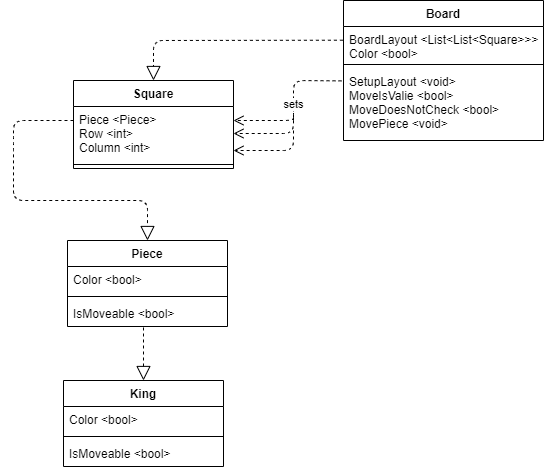
\includegraphics[width=10cm]{entitys.png}
		\caption{\label{pic:umlEntitys} UML-Diagramm der Entitys}
	\end{center}
\end{figure}
Das Diagramm zeigt die Schach-Logik im Kern unserer Clean Architecture, bzw. die Entitys. Das \texttt{Board} stellt das Schachbrett dar. Dieses besteht aus 64 \texttt{Squares}. Die Methode \texttt{SetupLayout} erstellt das Board und besetzt die richtigen Felder mit Pieces mit der entsprechenden Farbe.
Von den eigentlichen \texttt{Pieces} ist hier nur der König gezeigt, da die anderen Figuren genau wie er die Methode \texttt{IsMoveable} implementieren. 
Das Board bietet drei Methoden, von denen nur eine tatsächlich von weiteren Schichten verwendet wird: \texttt{MovePiece}. Die Methode überprüft mit \texttt{MoveIsVali} ob es sich um einen Validen Zug handelt. \texttt{MoveIsValid} ruft dabei die von Figuren implementierte Methode \texttt{IsMoveable} auf um zu überprüfen ob die Figur theoretisch in der Lage wäre den Zug durchzuführen (zB. kann der Läufer schräg dahin?). Ist der Zug möglich wird noch überprüft ob weitere Figuren im Weg stehen und ob der Zug sich selbst in Schach setzen würde (\texttt{MoveDoesNotCheck}). Ist alles überprüft, wird der Zug durchgeführt.

\section{Programmierprizipien}
\subsection{pros/cons/wieso wir?}
\subsection{SOLID}
\subsubsection{Single Resposibility Principle}
\subsubsection{Open/Closed Principle}
\subsubsection{Liskov' Substitution Principle}
\subsubsection{Interface Segregation Principle}
\subsubsection{Dependency Inversion Principle}
Auf Translator anwenden
\subsection{GRASP}
\subsubsection{Low Coupling}
\subsubsection{High Cohesion}
\subsection{DRY (Don't Repeat Yourself)}
Schon umgesetzt?


\section{Unit Testing}
\subsection{pros/cons/wieso wir?}
\subsection{ATRIP}
\subsection{Code Coverage}
\subsection{Mocking}

\section{Refactoring}
\subsection{Beispiele und Begründungen}
\subsection{Code Smells}

\section{Entwurfsmuster}
\subsection{Diagramme und Begründungen}

\section{Fazit}\label{sec:end}

\end{document}